\documentclass[12pt,a4paper,openany,oneside]{report}
\usepackage[utf8]{vietnam}
\usepackage{amsmath, amsthm, amssymb,amsxtra,latexsym,amscd,graphpap,makeidx}
\usepackage{pgf,tikz}
\usepackage{mathrsfs}
\usetikzlibrary{arrows}
\usepackage{float}
\usepackage{algorithm}
\usepackage{algpseudocode}
\usepackage{graphicx}
\usepackage{array,tabularx,longtable,multicol,indentfirst,fancyhdr}
\usepackage[mathscr]{eucal}
\usepackage[top=3.5cm, bottom=3.0cm, left=3.5cm, right=2cm]{geometry}
\usepackage{fancybox}
\usepackage{listings}
\usepackage{xcolor}
\usepackage[utf8]{inputenc}
\usepackage{hyperref}
\usepackage[strings]{underscore}

\usepackage{multirow}
\usepackage{booktabs}
\usepackage{enumitem}
\usepackage{multirow}
\usepackage{ragged2e}

% Định dạng màu listings
\definecolor{codegreen}{rgb}{0,0.5,0}
\definecolor{codegray}{rgb}{0.5,0.5,0.5}
\definecolor{codepurple}{rgb}{0.58,0,0.82}
\definecolor{codeblue}{rgb}{0,0,0.8}
\definecolor{backcolour}{rgb}{0.95,0.95,0.92}

% Định dạng code Assembly
\lstdefinestyle{assemblystyle}{
    backgroundcolor=\color{backcolour},
    commentstyle=\color{codegreen}, 
    keywordstyle=\color{codeblue}, 
    numberstyle=\tiny\color{codegray},
    stringstyle=\color{codepurple},
    basicstyle=\ttfamily\footnotesize,
    breakatwhitespace=true, 
    breaklines=true,
    captionpos=b,
    keepspaces=true,
    numbers=left,
    numbersep=5pt,
    showspaces=false,
    showstringspaces=false,
    showtabs=false,
    tabsize=2,
    language=[x86masm]Assembler, 
    morekeywords={proc, endp, model, stack, data, code, segment, ends, assume, offset, db, dw, dd, equ, org, include, macro, endm, rept, irp, irpc, exitm, local, public, extrn, group, label, align, even, if, else, endif, end, main, mov, lea, add, sub, inc, dec, mul, imul, div, idiv, cmp, test, and, or, xor, not, neg, shl, shr, sal, sar, rol, ror, rcl, rcr, jmp, call, ret, retf, retn, je, jz, jne, jnz, jg, jnle, jge, jnl, jl, jnge, jle, jng, ja, jnbe, jae, jnb, jb, jnae, jbe, jna, jc, jnc, jo, jno, js, jns, jp, jpe, jnp, jpo, jcxz, loop, loope, loopz, loopne, loopnz, int, into, iret, push, pop, pushf, popf, pusha, popa, std, cld, sti, cli, cmc, clc, stc, lahf, sahf, aaa, aad, aam, aas, daa, das, cbw, cwd, xlat, bound, enter, leave, nop, hlt, wait, lock, esc, rep, repe, repz, repne, repnz, xchg, les, lds, in, out, stosb, stosw, stosd, lodsb, lodsw, lodsd, scasb, scasw, scasd, movsb, movsw, movsd, cmpsb, cmpsw, cmpsd}, 
    inputencoding=utf8,
    extendedchars=true,
    literate={á}{{\\'a}}1 {é}{{\\'e}}1 {í}{{\\'i}}1 {ó}{{\\'o}}1 {ú}{{\\'u}}1
      {Á}{{\\'A}}1 {É}{{\\'E}}1 {Í}{{\\'I}}1 {Ó}{{\\'O}}1 {Ú}{{\\'U}}1
      {à}{{\`a}}1 {è}{{\`e}}1 {ì}{{\`i}}1 {ò}{{\`o}}1 {ù}{{\`u}}1
      {À}{{\`A}}1 {È}{{\\'E}}1 {Ì}{{\`I}}1 {Ò}{{\`O}}1 {Ù}{{\`U}}1
      {ä}{{\"a}}1 {ë}{{\"e}}1 {ï}{{\"i}}1 {ö}{{\"o}}1 {ü}{{\"u}}1
      {Ä}{{\"A}}1 {Ë}{{\"E}}1 {Ï}{{\"I}}1 {Ö}{{\"O}}1 {Ü}{{\"U}}1
      {â}{{\^a}}1 {ê}{{\^e}}1 {î}{{\^i}}1 {ô}{{\^o}}1 {û}{{\^u}}1
      {Â}{{\^A}}1 {Ê}{{\^E}}1 {Î}{{\^I}}1 {Ô}{{\^O}}1 {Û}{{\^U}}1
      {œ}{{\oe}}1 {Œ}{{\OE}}1 {æ}{{\ae}}1 {Æ}{{\AE}}1 {ß}{{\ss}}1
      {ç}{{\c c}}1 {Ç}{{\c C}}1 {ø}{{\o}}1 {å}{{\r a}}1 {Å}{{\r A}}1
      {ã}{{\~a}}1 {õ}{{\~o}}1 {Ã}{{\~A}}1 {Õ}{{\~O}}1
      {ñ}{{\~n}}1 {Ñ}{{\~N}}1 {¿}{{?`}}1 {¡}{{!`}}1
      {°}{{\textdegree}}1 {ð}{{\dh}}1 {Ð}{{\DH}}1 {þ}{{\th}}1 {Þ}{{\TH}}1
}
\lstset{style=assemblystyle} 

\renewcommand{\chaptername}{Chương}
\renewcommand\bibname{Tài liệu tham khảo}

\pagestyle{fancy}
\fancyhf{}
\fancyhead[L]{\nouppercase{\leftmark}} 
\fancyhead[R]{\thepage} 
\fancyfoot[C]{} 
\renewcommand{\headrulewidth}{0.4pt}
\renewcommand{\footrulewidth}{0pt} 

\begin{document}

\newgeometry{top=2.0cm,bottom=3.0cm,left=3.0cm,right=2.8cm}
\setlength{\fboxrule}{1.5pt}
\thisfancypage{\setlength{\fboxsep}{10pt}\setlength{\shadowsize}{0pt}\doublebox}{}

\begin{titlepage}
\fontsize{14pt}{14pt}\selectfont \baselineskip 0.65cm
\thispagestyle{empty}
\begin{center}
{HỌC VIỆN CÔNG NGHỆ BƯU CHÍNH VIỄN THÔNG}\\
\textbf{\MakeUppercase{KHOA CÔNG NGHỆ THÔNG TIN I}}\\
\centerline{--------------------o0o--------------------}  
\end{center}

\begin{figure}[H]
	\begin{center}
		
\includegraphics[width=6cm]{logo.png}
	\end{center}
\end{figure} 
 
\vspace{0.5cm}
\begin{center}
\textbf{\MakeUppercase{\LARGE \bf BÁO CÁO BÀI TẬP LỚN}}\\ 
\end{center} 



\vspace{0.1cm}
\begin{center}
	\textbf{Môn: Kiến trúc máy tính}\\[0.5cm]
	\textbf{Chủ đề: Thiết kế Balloon Shooting Game bằng Assembly}\\[0.5cm]
	\textbf{Giảng viên: Trần Tiến Công}
\end{center}

\vspace{1cm}
\hspace{3cm}
\begin{tabular}{ll}
	Nguyễn Trường Thái & B23DCCN747 \\
	Hà Duy Khánh & B23DCCN426 \\
	Vũ Quang Huy & B23DCCN412 \\
	Lê Huy Hải & B23DCCN272 \\
\end{tabular}

\vfill
\begin{center}
{{\bf Hà Nội, 5/2025}}
\end{center}
\end{titlepage}

\restoregeometry
\pagestyle{fancy}
\pagenumbering{roman}  
\fontsize{13pt}{13pt}\selectfont \baselineskip 0.75cm 

\newpage
\thispagestyle{empty}
\tableofcontents
\newpage


\listoffigures
\addcontentsline{toc}{chapter}{Danh sách hình vẽ}
\newpage


\newgeometry{top=3.0cm,bottom=3.0cm,left=3.0cm,right=2.8cm}
\pagestyle{plain}
\fontsize{13pt}{13pt}\selectfont \baselineskip 0.75cm 

\begin{center}
    \Large \textbf{BẢNG PHÂN CÔNG CÔNG VIỆC CHI TIẾT}
\end{center}

\addcontentsline{toc}{chapter}{Bảng phân công công việc chi tiết}

\vspace{0.5cm} 

{\setlength{\LTpre}{0pt} 
 \setlength{\LTpost}{0pt} 


\begin{longtable}{c p{0.25\textwidth} >{\RaggedRight\arraybackslash\setlist[itemize]{leftmargin=*, topsep=0pt, partopsep=0pt, itemsep=1pt, parsep=1pt}}p{0.35\textwidth} p{0.25\textwidth}}

\toprule
\textbf{Thứ tự} & \textbf{Nhiệm vụ} & \textbf{Phạm vi} & \textbf{Mục tiêu} \\
\midrule
\endfirsthead

\multicolumn{4}{c}{{\bfseries BẢNG PHÂN CÔNG CÔNG VIỆC CHI TIẾT}} \\ 
\toprule
\textbf{Thứ tự} & \textbf{Nhiệm vụ} & \textbf{Phạm vi} & \textbf{Mục tiêu} \\
\midrule
\endhead


\endfoot

\bottomrule
\endlastfoot

% --- Table Content --- 

% Person 1
\multirow{2}{*}{Khánh} 
  & Khởi tạo, Menu và Luồng Điều Khiển Chính Ban Đầu 
  & 
    \begin{itemize}
      \item \texttt{main proc}: Thiết lập ban đầu, khởi tạo biến, gọi hàm chính.
      \item \texttt{game\_menu proc}: Logic menu (hiển thị, chờ Enter), gọi \texttt{clear\_screen}, \texttt{show\_score}, chuyển tiếp sang \texttt{main\_loop}.
    \end{itemize}
  & Hiểu cách khởi động, menu hoạt động, chuyển vào vòng lặp chính. \\
\cmidrule{2-4} 

% Person 2
\multirow{3}{*}{Huy} 
  & Vòng Lặp Chính và Xử Lý Đầu Vào Người Chơi
  & 
    \begin{itemize}
      \item \texttt{main\_loop proc}: Cấu trúc vòng lặp chính, điều phối hàm con.
      \item \texttt{key\_pressed proc}: Xử lý phím W, S, Space, Left.
      \item \texttt{inside\_loop proc}: Cập nhật vị trí người chơi.
    \end{itemize}
  & Hiểu cách xử lý phím và cập nhật trạng thái người chơi. \\
\cmidrule{2-4}

% Person 3
\multirow{2}{*}{Thái} 
  & Logic Cốt Lõi Của Game, viết báo cáo LaTeX và biên dịch báo cáo nhóm
  & 
    \begin{itemize}
      \item \texttt{inside\_loop proc}: Kiểm tra thua (miss~$\geq$~5), va chạm (arrow\_pos==loon\_pos), cập nhật và vẽ mũi tên/bóng bay.
    \end{itemize}
  & Hiểu cơ chế gameplay: va chạm, di chuyển, điều kiện thắng/thua. \\
\cmidrule{2-4}

% Person 4
\multirow{3}{*}{Hải} 
  & Kết Thúc Game và Các Hàm Tiện Ích
  & 
    \begin{itemize}
      \item \texttt{game\_over proc}, \texttt{win\_game proc}: Thông báo, hỏi chơi lại.
      \item \texttt{show\_score proc}: Cập nhật chuỗi điểm.
      \item \texttt{clear\_screen proc}: Xóa màn hình.
    \end{itemize}
  & Hiểu xử lý kết thúc game và các hàm tiện ích. \\

% --- End Table Content --- 

\end{longtable}
}
\restoregeometry


\pagestyle{fancy}
\pagenumbering{arabic}  
\fontsize{13pt}{13pt}\selectfont \baselineskip 0.75cm 

\chapter{Giới Thiệu Tổng Quan Về Trò Chơi}
Đề tài "Game Bắn Bóng Bay (Balloon Shooting Game) bằng Assembly" được thực hiện với mục tiêu tìm hiểu và ứng dụng ngôn ngữ lập trình Assembly để xây dựng một trò chơi đơn giản. Trò chơi mô phỏng việc người chơi điều khiển một đối tượng để bắn các bóng bay di chuyển trên màn hình. Việc lựa chọn đề tài này xuất phát từ mong muốn được thực hành các kiến thức về lập trình cấp thấp, quản lý bộ nhớ, và tương tác phần cứng cơ bản thông qua việc phát triển một ứng dụng giải trí nhỏ.

Trò chơi được phát triển dựa trên một phiên bản mã nguồn mở và đã được nhóm chỉnh sửa, cải tiến để phù hợp với yêu cầu của bài tập lớn. Qua đó, nhóm đã có cơ hội làm quen với cấu trúc của một chương trình Assembly, cách xử lý đồ họa ký tự, và logic điều khiển trong game.



\chapter{Hướng Dẫn Cách Chơi Và Điều Khiển}
Trò chơi "Balloon Shooting Game" có cách điều khiển và luật chơi đơn giản như sau:
\begin{itemize}
    \item \textbf{Điều khiển người chơi:}
    \begin{itemize}
        \item Nhấn phím \textbf{W} để di chuyển người chơi lên trên.
        \item Nhấn phím \textbf{S} để di chuyển người chơi xuống dưới.
    \end{itemize}
    \item \textbf{Bắn mũi tên:}
    \begin{itemize}
        \item Nhấn phím \textbf{Space (phím cách)} để bắn mũi tên từ vị trí của người chơi sang phải.
    \end{itemize}
    \item \textbf{Mục tiêu trò chơi:}
    \begin{itemize}
        \item Người chơi cần bắn trúng các bóng bay đang di chuyển từ phải sang trái màn hình.
    \end{itemize}
    \item \textbf{Điều kiện thắng:}
    \begin{itemize}
        \item Bắn trúng \textbf{2} quả bóng bay (biến `hits` = 2). Đây là giá trị để dễ dàng kiểm thử, có thể tăng lên để trò chơi thử thách hơn.
    \end{itemize}
    \item \textbf{Điều kiện thua:}
    \begin{itemize}
        \item Để lọt \textbf{5} quả bóng bay (biến `miss` = 5). Tương tự như điều kiện thắng, giá trị này có thể được điều chỉnh.
    \end{itemize}
    \item \textbf{Chơi lại hoặc thoát:}
    \begin{itemize}
        \item Sau khi thắng hoặc thua, màn hình sẽ hiển thị tùy chọn chơi lại.
        \item Nhấn phím \textbf{Y} hoặc \textbf{y} để chơi lại.
        \item Nhấn phím \textbf{N} hoặc \textbf{n} để thoát khỏi trò chơi.
    \end{itemize}
    \item \textbf{Phím debug :}
    \begin{itemize}
        \item Trong một số phiên bản, phím mũi tên trái có thể được dùng để tăng số lần miss nhằm mục đích kiểm thử.
    \end{itemize}
\end{itemize}



\chapter{Kết Quả Thực Thi Và Hình Ảnh Minh Họa Trò Chơi}
Phần này trình bày một số hình ảnh minh họa giao diện và các trạng thái của trò chơi khi thực thi trên trình giả lập Emu8086.

\begin{figure}[H]
    \centering
    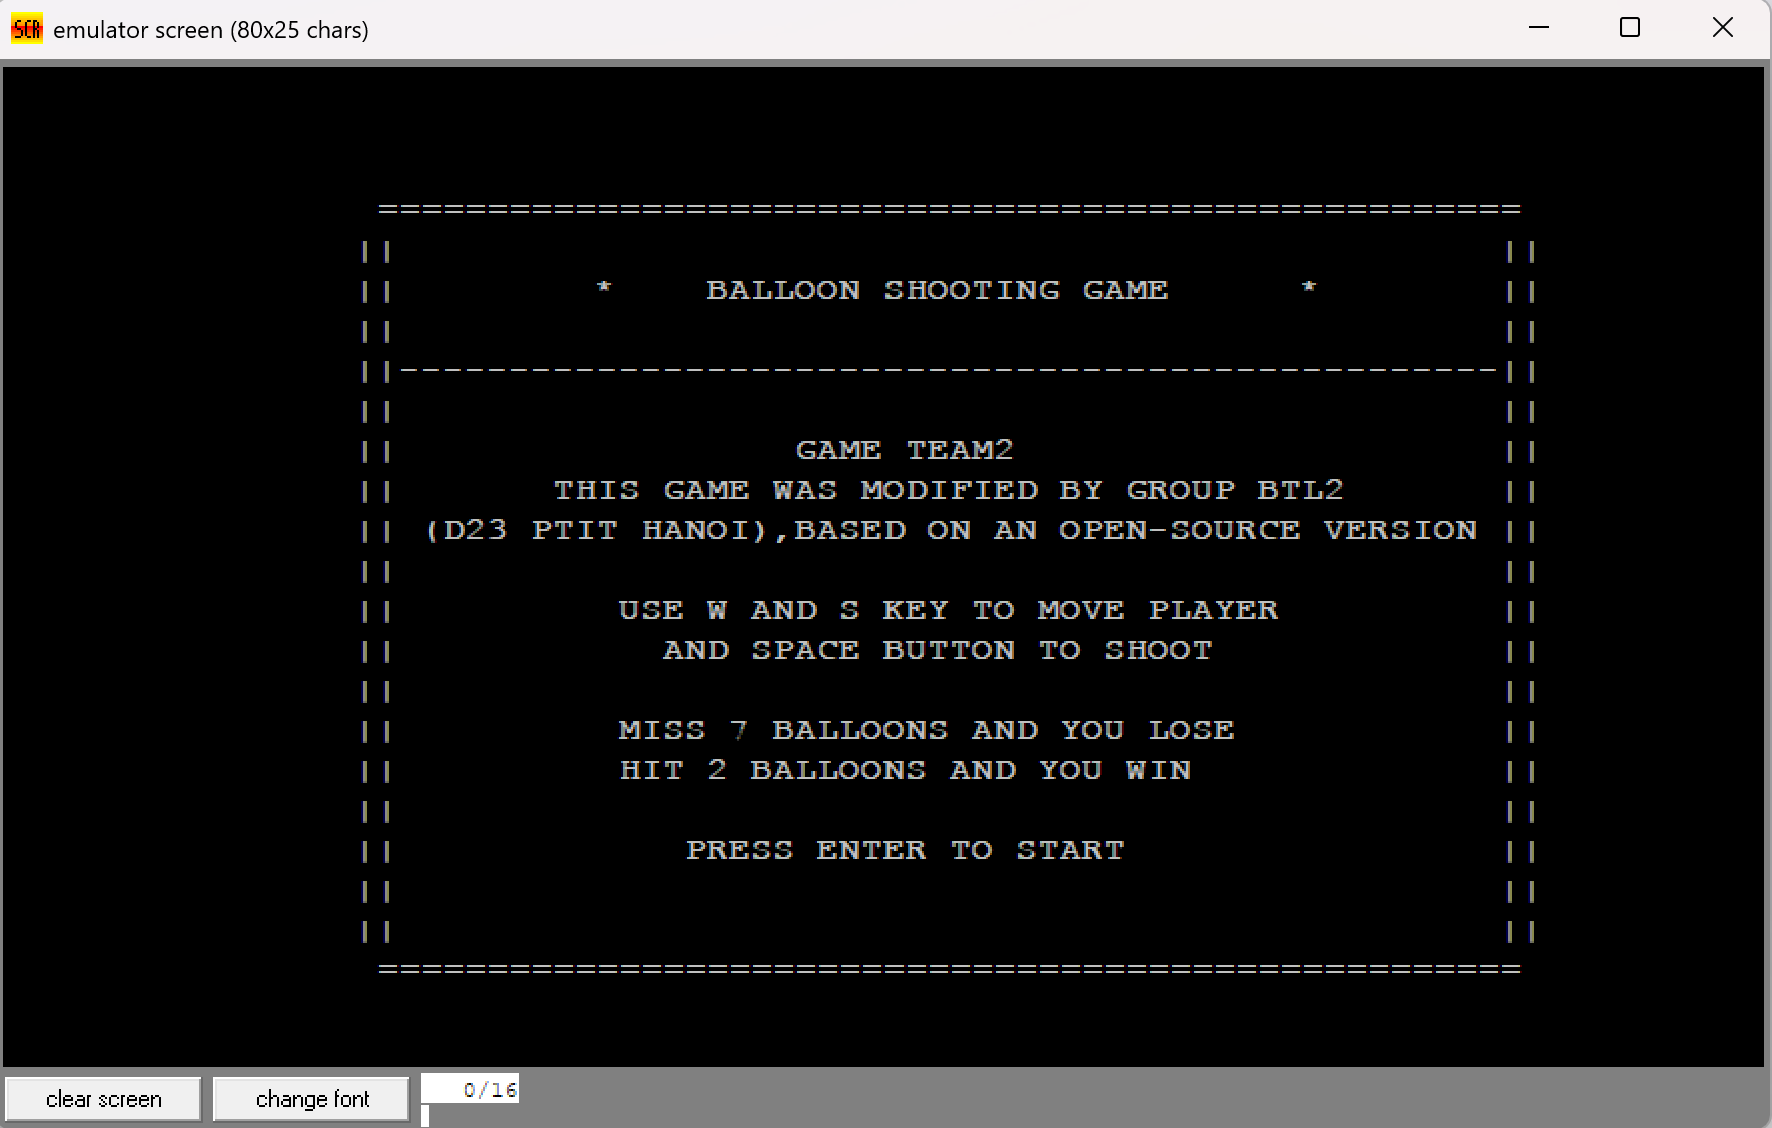
\includegraphics[width=0.8\textwidth]{game_menu.png}
    \caption{Giao diện menu chính của trò chơi.}
    \label{fig:game_menu}
\end{figure}


\begin{figure}[H]
    \centering
    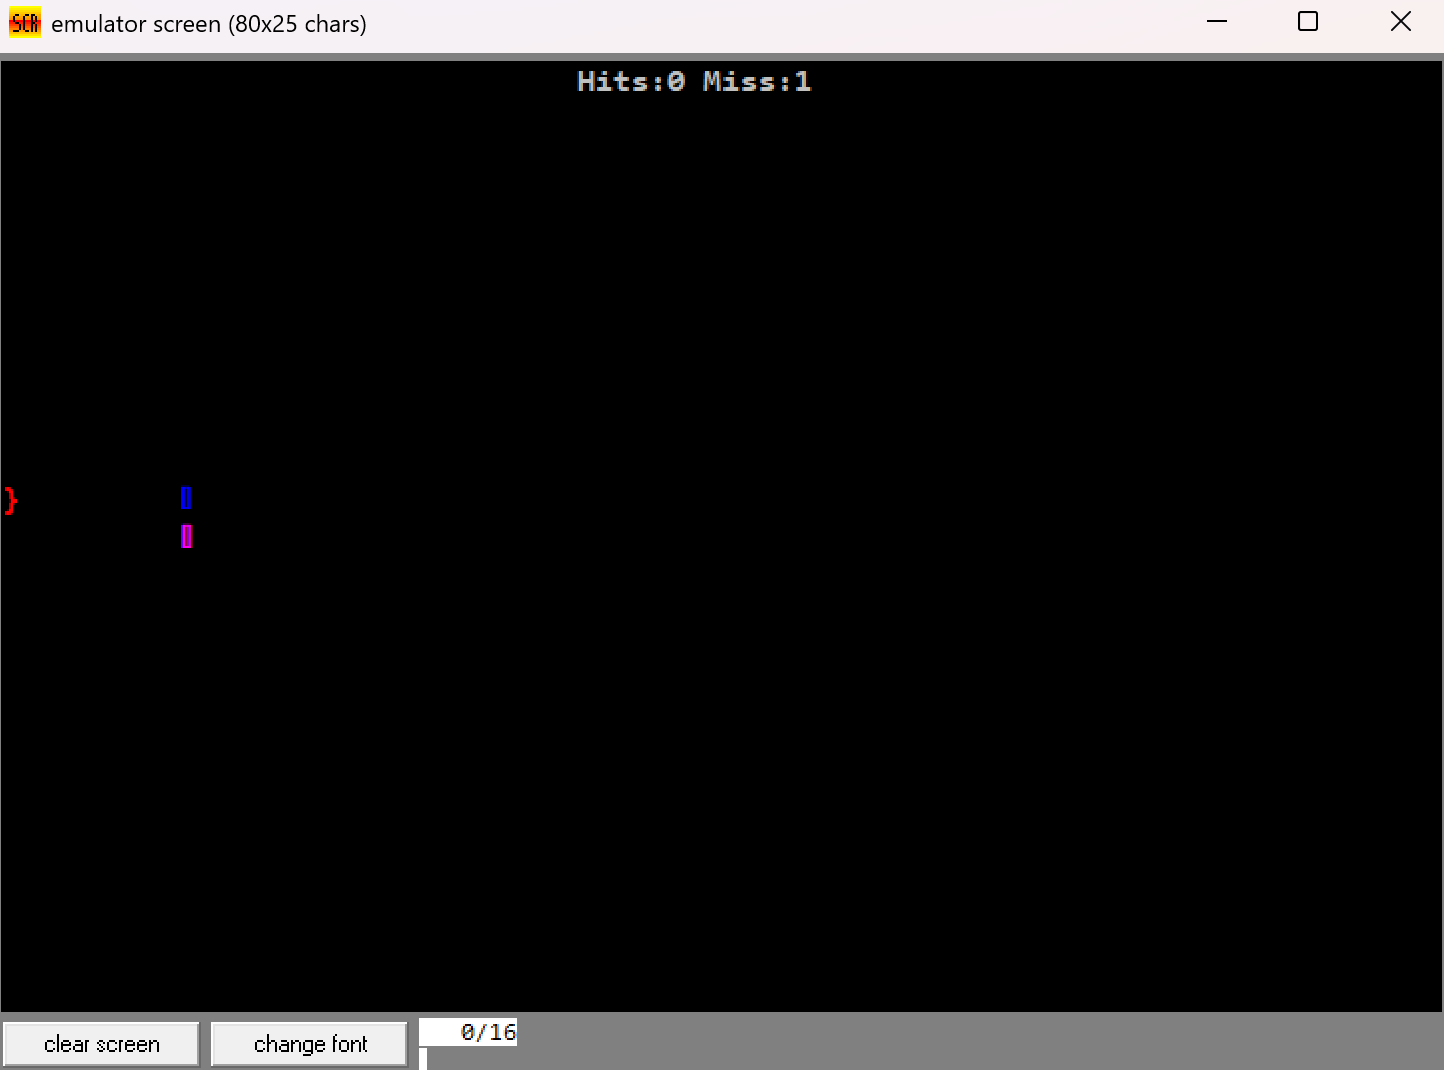
\includegraphics[width=0.8\textwidth]{play_game.png}
    \caption{Giao diện trong trò chơi.}
\end{figure}


\begin{figure}[H]
    \centering
    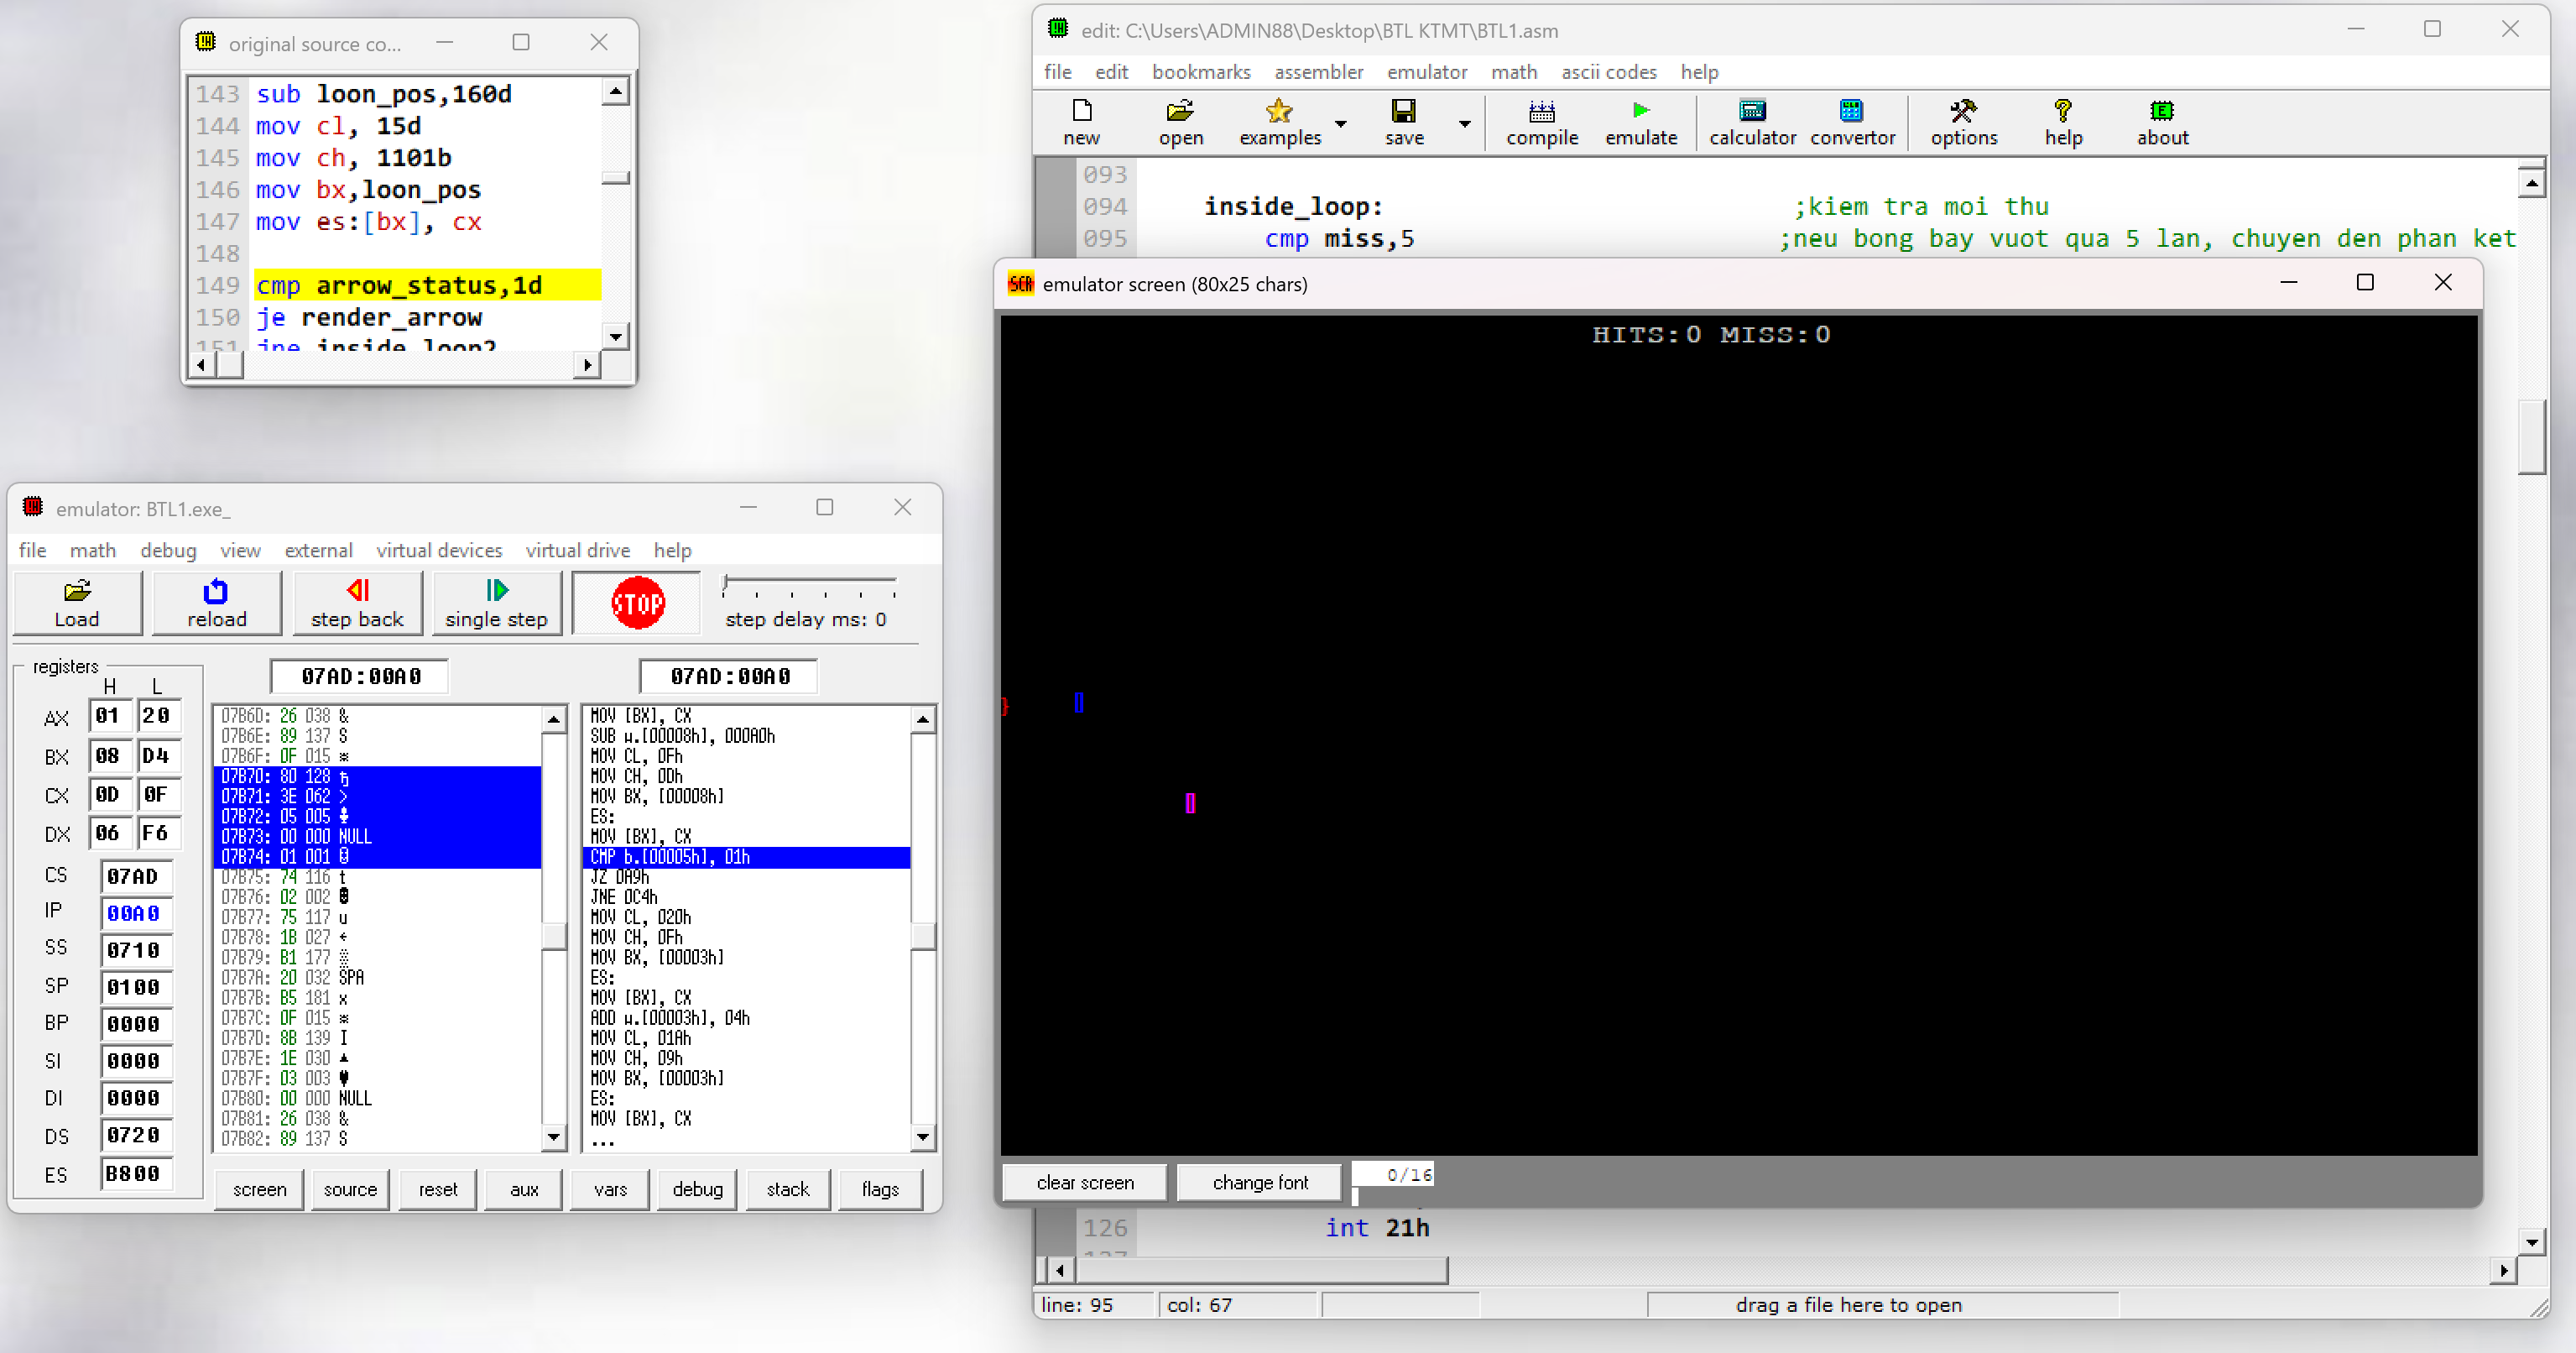
\includegraphics[width=1\textwidth]{full_emulator_view.png}
    \caption{Toàn cảnh trò chơi đang diễn ra trong trình giả lập Emu8086, bao gồm màn hình game, mã nguồn và các thanh ghi.}
    \label{fig:full_emulator_view}
\end{figure}

\begin{figure}[H]
    \centering
    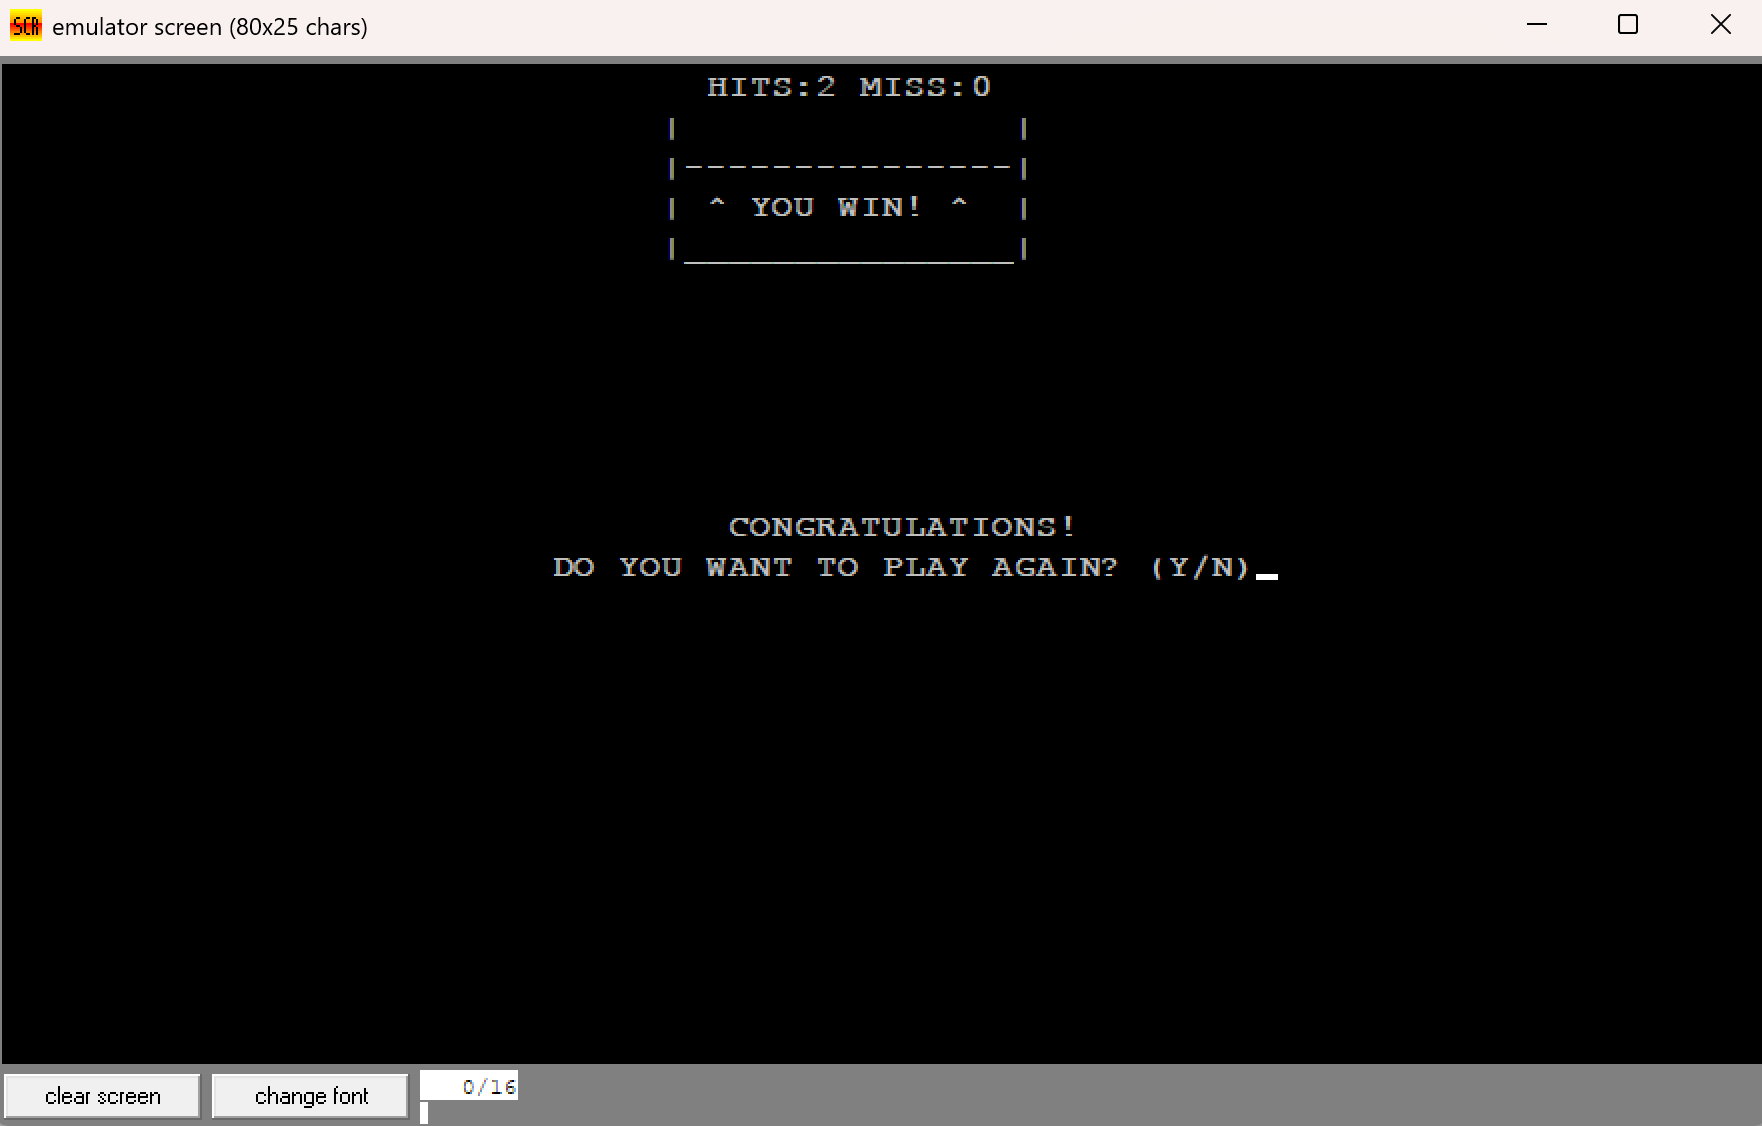
\includegraphics[width=0.8\textwidth]{game_win.png}
    \caption{Màn hình thông báo chiến thắng khi người chơi đạt đủ điểm.}
    \label{fig:game_win}
\end{figure}

\begin{figure}[H]
    \centering
    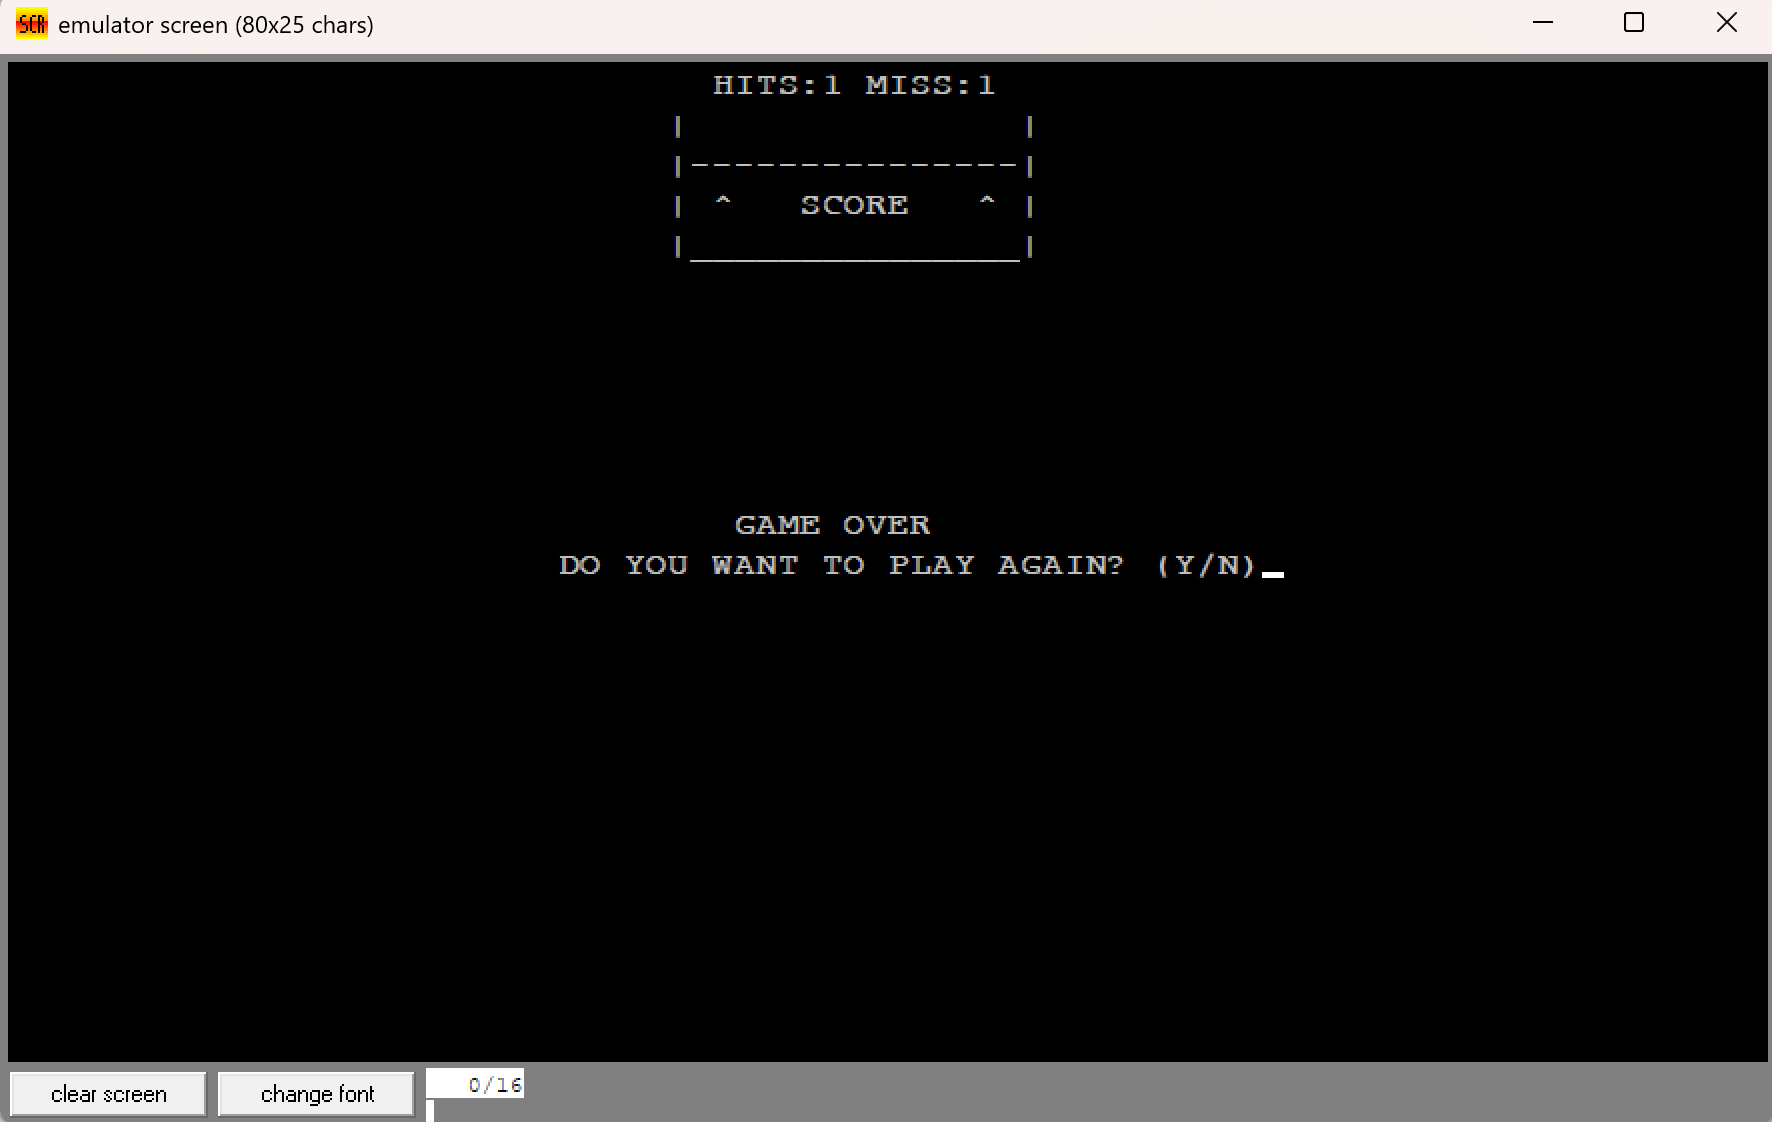
\includegraphics[width=0.8\textwidth]{game_over.png}
    \caption{Màn hình thông báo thua cuộc khi người chơi để lọt quá nhiều bóng bay.}
    \label{fig:game_over}
\end{figure}

Các hình ảnh trên cho thấy các giao diện cơ bản của trò chơi, từ lúc bắt đầu, trong quá trình chơi, cho đến khi kết thúc một lượt chơi với kết quả thắng hoặc thua. Giao diện được thiết kế đơn giản bằng các ký tự đồ họa trong chế độ text mode của Assembly.


\chapter{Phân Tích Cấu Trúc Mã Nguồn Balloon Shooting Game}
Chương trình Balloon Shooting Game được viết bằng ngôn ngữ Assembly cho vi xử lý 8086, sử dụng trình biên dịch EMU8086. Cấu trúc tổng quan của mã nguồn bao gồm các thành phần chính sau:
\begin{itemize}
    \item \textbf{.model large}: Khai báo mô hình bộ nhớ lớn (large memory model). Mô hình này cho phép chương trình sử dụng nhiều đoạn mã (code segments) và nhiều đoạn dữ liệu (data segments) khác nhau, mỗi đoạn có thể lên tới 64KB. Điều này cung cấp không gian địa chỉ rộng hơn cho các chương trình phức tạp.
    \item \textbf{.stack 100h}: Dành riêng một vùng nhớ có kích thước 100h (256 bytes) cho ngăn xếp (stack). Ngăn xếp được sử dụng để lưu trữ địa chỉ trả về của các thủ tục, các biến cục bộ, và các tham số truyền cho thủ tục.
    \item \textbf{.data}: Khu vực khai báo các biến và hằng số mà chương trình sử dụng. Trong trò chơi này, phần .data chứa các biến lưu trữ vị trí của người chơi, mũi tên, bóng bay; trạng thái của các đối tượng; điểm số (số lần bắn trúng, số lần bắn trượt); và các chuỗi ký tự dùng để hiển thị thông báo trên màn hình (menu game, thông báo thắng/thua, điểm số).
    \item \textbf{.code}: Chứa toàn bộ mã lệnh thực thi của chương trình. Phần này bao gồm thủ tục chính (main proc) là điểm bắt đầu của chương trình, cùng với các thủ tục con và các nhãn (labels) khác để thực hiện các chức năng cụ thể của trò chơi như hiển thị menu, xử lý sự kiện bàn phím, di chuyển đối tượng, kiểm tra va chạm, cập nhật điểm số, và hiển thị màn hình kết thúc game.
\end{itemize}


\section*{Sơ đồ luồng chương trình}

\begin{itemize}[leftmargin=*, itemsep=1pt, parsep=1pt]
    \item \texttt{main proc} 
    \begin{itemize}
        \item \texttt{game\_menu} (Quản lý menu)
        \begin{itemize}
            \item Hiển thị menu.
            \item Chờ nhấn Enter.
            \item Gọi \texttt{clear\_screen proc}.
            \item Gọi \texttt{show\_score proc}.
        \end{itemize}
        \item \texttt{main\_loop} (Vòng lặp chính)
        \begin{itemize}
            \item Kiểm tra phím nhấn.
            \begin{itemize}
                \item \texttt{key\_pressed}: Xử lý phím (W, S, Space, Left).
            \end{itemize}
            \item \texttt{inside\_loop} (Logic game cốt lõi)
            \begin{itemize}
                \item Kiểm tra thua (\texttt{miss >= 5}).
                \item Kiểm tra va chạm (\texttt{arrow\_pos == loon\_pos}).
                \item Cập nhật vị trí: người chơi, mũi tên, bóng bay.
                \item Vẽ đối tượng.
            \end{itemize}
            \item \texttt{game\_over} (Xử lý thua)
            \begin{itemize}
                \item Hiển thị thông báo thua.
                \item Hỏi chơi lại (Y/N).
            \end{itemize}
            \item \texttt{win\_game} (Xử lý thắng)
            \begin{itemize}
                \item Hiển thị thông báo thắng.
                \item Hỏi chơi lại (Y/N).
            \end{itemize}
        \end{itemize}
        \item \texttt{show\_score proc} (Tiện ích hiển thị điểm)
        \begin{itemize}
            \item Cập nhật chuỗi điểm số.
        \end{itemize}
        \item \texttt{clear\_screen proc} (Tiện ích xóa màn hình)
        \begin{itemize}
            \item Xóa màn hình console.
        \end{itemize}
    \end{itemize}
\end{itemize}

Tổng quan, chương trình được tổ chức thành các module chức năng thông qua các thủ tục và nhãn, giúp mã nguồn dễ đọc và quản lý hơn.

\chapter{Phân Tích Chi Tiết Chức Năng }
Phần này mô tả chi tiết các thủ tục, nhãn và biến quan trọng trong mã nguồn.

\section{Chi tiết các Thủ tục Chính (Procedures)}
\begin{itemize}
    \item \textbf{main proc}: Đây là thủ tục chính, điểm khởi đầu của chương trình. Nó thực hiện việc khởi tạo các đoạn dữ liệu (DS) và đoạn màn hình (ES), sau đó nhảy đến nhãn `game_menu` để hiển thị menu bắt đầu trò chơi.
    \item \textbf{show\_score proc}: Thủ tục này chịu trách nhiệm hiển thị điểm số hiện tại của người chơi, bao gồm số lần bắn trúng (Hits) và số lần bắn trượt (Miss). Điểm số được định dạng thành chuỗi "Hits:X Miss:Y" và lưu vào biến `state_buf`.
    \item \textbf{clear\_screen proc}: Thủ tục này dùng để xóa toàn bộ nội dung trên màn hình. Nó sử dụng ngắt 10h của BIOS với AH=0, AL=3 (chế độ văn bản 80x25 màu).
\end{itemize}



\section{Giải thích các Biến (Variables) Dữ liệu Chính}
\begin{itemize}
    \item \textbf{hits dw 0d}: Lưu số lần người chơi bắn trúng bóng bay. Điều kiện thắng là khi `hits` đạt 2 (trong phiên bản test, có thể tăng lên để khó hơn).
    \item \textbf{miss dw 0d}: Lưu số lần người chơi bắn trượt bóng bay (bóng bay bay qua màn hình). Điều kiện thua là khi `miss` đạt 5 (trong phiên bản test, có thể là 1 hoặc 7 tùy theo mô tả, mã nguồn ghi là 5).
    \item \textbf{player\_pos dw 1760d}: Lưu vị trí (offset trong bộ nhớ video) của người chơi trên màn hình. Giá trị ban đầu là 1760d.
    \item \textbf{arrow\_pos dw 0d}: Lưu vị trí của mũi tên. Giá trị 0d có nghĩa là mũi tên chưa được bắn hoặc đã biến mất.
    \item \textbf{loon\_pos dw 3860d}: Lưu vị trí của bóng bay. Giá trị ban đầu là 3860d (bên phải màn hình).
    \item \textbf{arrow\_status db 0d}: Trạng thái của mũi tên. 0d nghĩa là mũi tên sẵn sàng để bắn, 1d nghĩa là mũi tên đang bay.
    \item \textbf{arrow\_limit dw 22d}: Giới hạn di chuyển của mũi tên. Khi `arrow_pos` vượt qua `player_pos + arrow_limit`, mũi tên sẽ biến mất. Giá trị 22d là một khoảng cách ngắn, có thể điều chỉnh.
    \item \textbf{direction db 0d}: Lưu hướng di chuyển mà người chơi yêu cầu (8d cho lên, 2d cho xuống, 0d là không di chuyển).
    \item \textbf{state\_buf db '00:0:0:0:0:0:00:00\$'}: Bộ đệm để lưu chuỗi điểm số hiển thị.
    \item \textbf{game\_over\_str, game\_start\_str, win\_str}: Các chuỗi ký tự dùng để hiển thị thông báo tương ứng.
\end{itemize}



\section{Phân tích các Nhãn (Labels) Quan trọng}
\begin{itemize}
    \item \textbf{game\_menu}: Hiển thị giao diện menu chính của trò chơi, bao gồm tên game, thông tin nhóm phát triển, hướng dẫn cách chơi cơ bản. Chờ người chơi nhấn phím Enter để bắt đầu.
\begin{lstlisting}[caption={Mã nguồn nhãn game_menu}, basicstyle=\ttfamily\footnotesize, numbers=left, numberstyle=\tiny, stepnumber=1, numbersep=5pt, breaklines=true, language={[x86masm]Assembler}]
game_menu:
    mov ah,09h
    mov dh,0
    mov dx, offset game_start_str ;tro den chuoi bat dau tro choi
    int 21h                       ;goi ngat 21h de hien thi chuoi
;nhan dau vao tu nguoi choi
    input2:
        mov ah,1
        int 21h
        cmp al,13d      ;so sanh ky tu nhap voi ma phim Enter
        jne input2      ;neu khong phai Enter thi cho nhap lai
        call clear_screen  ;goi thu tuc xoa man hinh
        
        lea bx,state_buf   ;gan dia chi diem so vao bx
        call show_score    ;goi thu tuc hien thi diem so
        lea dx,state_buf   ;gan dia chi diem vao Dx de hien thi 
        mov ah,09h
        int 21h            ;goi ngat 21h de hien thi diem
         
        mov ah,2           ;ham 02h-xuat mot ky tu ra man hinh
        mov dl, 0dh
        int 21h
        jmp main_loop      ;nhay den vong lap chinh tro choi
\end{lstlisting} 
    \item \textbf{main\_loop}: Vòng lặp chính của trò chơi. Trong mỗi vòng lặp, chương trình kiểm tra xem có phím nào được nhấn không (qua ngắt 16h). Nếu có, nhảy đến `key_pressed` để xử lý. Nếu không, tiếp tục thực hiện logic trong `inside_loop`.
\begin{lstlisting}[caption={Mã nguồn nhãn game_loop}, basicstyle=\ttfamily\footnotesize, numbers=left, numberstyle=\tiny, stepnumber=1, numbersep=5pt, breaklines=true, language={[x86masm]Assembler}]
main_loop:      ;Cap nhat logic va hien thi moi thu
    mov ah,1h
    int 16h         ;Kiem tra neu co phim duoc nhan
    jnz key_pressed ;Neu co,nhay den key_pressed
    jmp inside_loop ;Neu khong,nhay den inside_loop
\end{lstlisting} 
    \item \textbf{inside\_loop}: Thực hiện các công việc cốt lõi của game trong mỗi frame: kiểm tra điều kiện thua (miss >= 5), kiểm tra va chạm giữa mũi tên và bóng bay, cập nhật vị trí người chơi dựa trên biến `direction`, ẩn mũi tên nếu vượt quá giới hạn, kiểm tra bóng bay có bay qua màn hình không. Sau đó gọi các nhãn để vẽ lại đối tượng.
\begin{lstlisting}[caption={Mã nguồn nhãn inside_loop}, basicstyle=\ttfamily\footnotesize, numbers=left, numberstyle=\tiny, stepnumber=1, numbersep=5pt, breaklines=true, language={[x86masm]Assembler}]
inside_loop:         ;kiem tra moi thu
    cmp miss,5          ; dieu kien thua,thay doi tuy y
    jge game_over
        
    mov dx,arrow_pos      ;kiem tra va cham
    cmp dx, loon_pos
    je hit
        
    cmp direction,8d      ;cap nhat vi tri nguoi choi
    je player_up
    cmp direction,2d      ;len hoac xuong dua tren bien huong
    je player_down
        
    mov dx,arrow_limit    ;an mui ten 
    cmp arrow_pos, dx
    jge hide_arrow
        
    cmp loon_pos, 0d      ;kiem tra bong bay vuot qua
    jle miss_loon
    jne render_loon 
\end{lstlisting} 
    \item \textbf{hit}: Được gọi khi mũi tên bắn trúng bóng bay. Thủ tục này phát âm thanh nhỏ, tăng biến `hits`, cập nhật và hiển thị lại điểm số. Kiểm tra nếu `hits` đạt 2 thì chuyển đến màn hình thắng (`win_game`). Sau đó, gọi `fire_loon` để tạo bóng bay mới.
\begin{lstlisting}[caption={Mã nguồn nhãn hit}, basicstyle=\ttfamily\footnotesize, numbers=left, numberstyle=\tiny, stepnumber=1, numbersep=5pt, breaklines=true, language={[x86masm]Assembler}]
hit:                 
    mov ah,2           ;in ra ky tu } tren man hinh
    mov dx, 7d
    int 21h 
            
    inc hits           ;cap nhat diem so

    lea bx,state_buf   ;hien thi diem so ngay lap tuc
    call show_score 
    lea dx,state_buf
    mov ah,09h
    int 21h

    mov ah,2          ;xuong dong
    mov dl, 0dh
    int 21h

    cmp hits, 2       ;dieu kien thang,thay doi tuy y
    je win_game

    jmp fire_loon     ;bong bay moi xuat hien
\end{lstlisting} 
    \item \textbf{render\_loon}: Di chuyển bóng bay từ phải sang trái và vẽ lại bóng bay ở vị trí mới. Trước đó, xóa hình ảnh bóng bay ở vị trí cũ.
\begin{lstlisting}[caption={Mã nguồn nhãn render_loon}, basicstyle=\ttfamily\footnotesize, numbers=left, numberstyle=\tiny, stepnumber=1, numbersep=5pt, breaklines=true, language={[x86masm]Assembler}]
render_loon:           ;ve bong bay
    mov cl, ' '        ;an bong bay cu
    mov ch, 1111b
    mov bx,loon_pos 
    mov es:[bx], cx
                
    sub loon_pos,160d   ;va ve bong bay moi o vi tri moi
    mov cl, 15d
    mov ch, 1101b
    mov bx,loon_pos 
    mov es:[bx], cx
            
    cmp arrow_status,1d ;kiem tra xem co mui ten nao de ve khong
    je render_arrow
    jne inside_loop2 
\end{lstlisting} 
    \item \textbf{render\_arrow}: Nếu mũi tên đang được bắn (`arrow_status = 1`), thủ tục này di chuyển mũi tên sang phải và vẽ lại mũi tên ở vị trí mới. Trước đó, xóa hình ảnh mũi tên ở vị trí cũ.
\begin{lstlisting}[caption={Mã nguồn nhãn render_arrow}, basicstyle=\ttfamily\footnotesize, numbers=left, numberstyle=\tiny, stepnumber=1, numbersep=5pt, breaklines=true, language={[x86masm]Assembler}]
render_arrow:           ;ve mui ten
    mov cl, ' '
    mov ch, 1111b
    mov bx,arrow_pos    ;an vi tri cu
    mov es:[bx], cx
                
    add arrow_pos,4d    ;ve vi tri moi
    mov cl, 26d
    mov ch, 1001b
    mov bx,arrow_pos 
    mov es:[bx], cx
\end{lstlisting} 
    \item \textbf{player\_up}: Di chuyển người chơi lên trên một khoảng cách nhất định bằng cách trừ giá trị `player_pos` đi 160 (một dòng trên màn hình text mode). Đặt lại `direction` về 0.
\begin{lstlisting}[caption={Mã nguồn nhãn player_up}, basicstyle=\ttfamily\footnotesize, numbers=left, numberstyle=\tiny, stepnumber=1, numbersep=5pt, breaklines=true, language={[x86masm]Assembler}]
player_up:                 
    mov cl, ' '             ;an vi tri cu cua nguoi choi
    mov ch, 1111b
    mov bx,player_pos 
    mov es:[bx], cx
    
    sub player_pos, 160d    ;dat vi tri moi cho nguoi choi
    mov direction, 0    
    jmp inside_loop2        ;no se duoc ve trong vong lap chinh
\end{lstlisting} 
    \item \textbf{player\_down}: Di chuyển người chơi xuống dưới một khoảng cách nhất định bằng cách cộng giá trị `player_pos` thêm 160. Đặt lại `direction` về 0.
\begin{lstlisting}[caption={Mã nguồn nhãn player_down}, basicstyle=\ttfamily\footnotesize, numbers=left, numberstyle=\tiny, stepnumber=1, numbersep=5pt, breaklines=true, language={[x86masm]Assembler}]
player_down:
    mov cl, ' '          ;giong nhu player_up
    mov ch, 1111b        ;an cai cu va dat vi tri moi
    mov bx,player_pos 
    mov es:[bx], cx
    
    add player_pos,160d  ;va vong lap chinh se ve no
    mov direction, 0
    jmp inside_loop2
\end{lstlisting} 
    \item \textbf{key\_pressed}: Xử lý các phím người chơi nhấn. Kiểm tra mã phím (AH) để xác định hành động: phím 'W' (11h) gọi `upKey`, phím 'S' (1Fh) gọi `downKey`, phím Space (39h) gọi `spaceKey` (bắn tên), phím mũi tên trái (4Bh) dùng để debug (tăng `miss`).
\begin{lstlisting}[caption={Mã nguồn nhãn key_pressed}, basicstyle=\ttfamily\footnotesize, numbers=left, numberstyle=\tiny, stepnumber=1, numbersep=5pt, breaklines=true, language={[x86masm]Assembler}]
key_pressed:           ;phan xu ly dau vao
    mov ah,0
    int 16h

    cmp ah,11h ;11h la Scan Code (hex) cua W     
    je upKey   ;chuyen den upKey neu duoc nhan
    cmp ah,1Fh ;1Fh la Scan Code (hex) cua S    
    je downKey ;chuyen den downKey neu duoc nhan
    
    cmp ah,39h      ;chuyen den spaceKey neu nut space duoc nhan
    je spaceKey
    
    cmp ah,4Bh      ;chuyen den leftKey (dung de debug)
    je leftKey
    jmp inside_loop ;neu khong nhan nut nao,nhay den inside_loop
\end{lstlisting}    
    \item \textbf{upKey}: Đặt biến `direction` thành 8 (hướng lên).
\begin{lstlisting}[caption={Mã nguồn nhãn upKey}, basicstyle=\ttfamily\footnotesize, numbers=left, numberstyle=\tiny, stepnumber=1, numbersep=5pt, breaklines=true, language={[x86masm]Assembler}]
upKey:       ;dat huong di chuyen cua nguoi choi len tren
    mov direction, 8d
    jmp inside_loop
\end{lstlisting}    
    \item \textbf{downKey}: Đặt biến `direction` thành 2 (hướng xuống).
\begin{lstlisting}[caption={Mã nguồn nhãn downKey}, basicstyle=\ttfamily\footnotesize, numbers=left, numberstyle=\tiny, stepnumber=1, numbersep=5pt, breaklines=true, language={[x86masm]Assembler}]
downKey:      ;dat huong di chuyen cua nguoi choi xuong duoi
    mov direction, 2d   
    jmp inside_loop
\end{lstlisting} 
    \item \textbf{spaceKey} / \textbf{fire\_arrow}: Nếu mũi tên chưa được bắn (`arrow_status = 0`), thủ tục này sẽ bắn mũi tên. Nó đặt vị trí ban đầu của mũi tên (`arrow_pos`) bằng vị trí hiện tại của người chơi (`player_pos`), đặt giới hạn di chuyển của mũi tên (`arrow_limit`), và cập nhật `arrow_status` thành 1 (đang bắn).
\begin{lstlisting}[caption={Mã nguồn nhãn spaceKey/fire_arrow}, basicstyle=\ttfamily\footnotesize, numbers=left, numberstyle=\tiny, stepnumber=1, numbersep=5pt, breaklines=true, language={[x86masm]Assembler}]
spaceKey:               ;ban mui ten
    cmp arrow_status,0
    je  fire_arrow
    jmp inside_loop

fire_arrow:              ;dat vi tri mui ten tai vi tri nguoi choi
    mov dx, player_pos   ;de mui ten ban tu vi tri nguoi choi
    mov arrow_pos, dx
    
    mov dx,player_pos     ;khi ban mui ten, no cung dat gioi han
    mov arrow_limit, dx   ;cua mui ten, noi ma no se bi an
    add arrow_limit, 22d  ;150
    
    mov arrow_status, 1d   ;dat trang thai mui ten,ngan chan ban nhieu lan
    jmp inside_loop        
\end{lstlisting} 
    \item \textbf{miss\_loon}: Được gọi khi bóng bay bay qua hết màn hình mà không bị bắn trúng. Tăng biến `miss`, cập nhật và hiển thị điểm số. Sau đó gọi `fire_loon` để tạo bóng bay mới.
\begin{lstlisting}[caption={Mã nguồn nhãn miss_loon}, basicstyle=\ttfamily\footnotesize, numbers=left, numberstyle=\tiny, stepnumber=1, numbersep=5pt, breaklines=true, language={[x86masm]Assembler}]
miss_loon:
    add miss,1           ;cap nhat diem so
    lea bx,state_buf     ;hien thi diem so
    call show_score 
    lea dx,state_buf
    mov ah,09h
    int 21h
                         ;xuong dong
    mov ah,2
    mov dl, 0dh
    int 21h
jmp fire_loon
\end{lstlisting} 
    \item \textbf{fire\_loon}: Tạo một bóng bay mới bằng cách đặt lại vị trí `loon_pos` về giá trị ban đầu (3860d, ở biên phải màn hình) và đặt `loon_status` thành 1.
\begin{lstlisting}[caption={Mã nguồn nhãn fire_loon}, basicstyle=\ttfamily\footnotesize, numbers=left, numberstyle=\tiny, stepnumber=1, numbersep=5pt, breaklines=true, language={[x86masm]Assembler}]
fire_loon:              ;ban bong bay moi
    mov loon_status, 1d
    mov loon_pos, 3860d     ;3990d
    jmp render_loon
\end{lstlisting} 
    \item \textbf{hide\_arrow}: Khi mũi tên bay đến giới hạn (`arrow_limit`), thủ tục này sẽ ẩn mũi tên bằng cách vẽ ký tự rỗng tại vị trí đó và đặt `arrow_status` về 0 (sẵn sàng bắn).
\begin{lstlisting}[caption={Mã nguồn nhãn hide_arrow}, basicstyle=\ttfamily\footnotesize, numbers=left, numberstyle=\tiny, stepnumber=1, numbersep=5pt, breaklines=true, language={[x86masm]Assembler}]
hide_arrow:
    mov arrow_status, 0      ;an mui ten
    mov cl, ' '
    mov ch, 1111b
    mov bx,arrow_pos 
    mov es:[bx], cx
    
    cmp loon_pos, 0d 
    jle miss_loon
    jne render_loon 
    jmp inside_loop2
\end{lstlisting} 
    \item \textbf{game\_over}: Hiển thị màn hình thông báo thua cuộc. Xóa các đối tượng game khỏi màn hình. Reset lại các biến game về giá trị ban đầu. Hỏi người chơi có muốn chơi lại không (Y/N). Nếu chọn 'Y' hoặc 'y', gọi `play_again`. Nếu chọn 'N' hoặc 'n', gọi `exit_game`.
\begin{lstlisting}[caption={Mã nguồn nhãn game_over}, basicstyle=\ttfamily\footnotesize, numbers=left, numberstyle=\tiny, stepnumber=1, numbersep=5pt, breaklines=true, language={[x86masm]Assembler}]
game_over:     
    mov cl, ' '         ; an bong bay
    mov ch, 1111b 
    mov bx, loon_pos  
    mov es:[bx], cx  
    
    mov cl, ' '         ; an mui ten
    mov ch, 1111b 
    mov bx, arrow_pos                      
    mov es:[bx], cx
          
    mov cl, ' '         ; an nguoi choi
    mov ch, 1111b 
    mov bx, player_pos  
    mov es:[bx], cx    
    
    mov ah, 09h         ; in chu "Game Over"
    mov dx, offset game_over_str
    int 21h
    
    ; reset bien
    mov miss, 0d
    mov hits, 0d
    mov player_pos, 1760d
    mov arrow_pos, 0d
    mov arrow_status, 0d 
    mov arrow_limit, 22d
    mov loon_pos, 3860d
    mov loon_status, 0d
    mov direction, 0d
\end{lstlisting} 
    \item \textbf{win\_game}: Hiển thị màn hình thông báo thắng cuộc. Xóa các đối tượng game. Reset biến. Hỏi người chơi có muốn chơi lại không (Y/N).
\begin{lstlisting}[caption={Mã nguồn nhãn win_game}, basicstyle=\ttfamily\footnotesize, numbers=left, numberstyle=\tiny, stepnumber=1, numbersep=5pt, breaklines=true, language={[x86masm]Assembler}]
win_game:
    mov ah, 09h         ; in chu "You Win"
    mov dx, offset win_str
    int 21h

    ; an mui ten
    mov cl, ' '
    mov ch, 1111b
    mov bx, arrow_pos
    mov es:[bx], cx

    ; an nguoi choi
    mov cl, ' '
    mov ch, 1111b
    mov bx, player_pos
    mov es:[bx], cx

    ; reset bien
    mov miss, 0d
    mov hits, 0d
    mov player_pos, 1760d
    mov arrow_pos, 0d
    mov arrow_status, 0d
    mov arrow_limit, 22d
    mov loon_pos, 3860d
    mov loon_status, 0d
    mov direction, 0d
\end{lstlisting} 
    \item \textbf{play\_again}: Xóa màn hình và nhảy về `main_loop` để bắt đầu lượt chơi mới.
\begin{lstlisting}[caption={Mã nguồn nhãn play_again}, basicstyle=\ttfamily\footnotesize, numbers=left, numberstyle=\tiny, stepnumber=1, numbersep=5pt, breaklines=true, language={[x86masm]Assembler}]
play_again:            ; choi lai
    call clear_screen  ; xoa man hinh
    jmp main_loop      ; quay lai vong lap chinh
\end{lstlisting}
    \item \textbf{exit\_game}: Kết thúc chương trình bằng ngắt 21h với AH=4Ch.
\begin{lstlisting}[caption={Mã nguồn nhãn exit_game}, basicstyle=\ttfamily\footnotesize, numbers=left, numberstyle=\tiny, stepnumber=1, numbersep=5pt, breaklines=true, language={[x86masm]Assembler}]
exit_game:             ; thoat game
    mov ah,4Ch         ; ham thoat DOS
    int 21h
\end{lstlisting}
\end{itemize}





\chapter{Tổng Kết, Đánh Giá Và Hướng Phát Triển}
Qua quá trình thực hiện bài tập lớn "Game Bắn Bóng Bay (Balloon Shooting Game) bằng Assembly", nhóm đã đạt được những kết quả nhất định. Trước hết, nhóm đã tìm hiểu và nắm vững hơn các kiến thức cơ bản về lập trình Assembly cho vi xử lý 8086, bao gồm cấu trúc chương trình, cách sử dụng các thanh ghi, tập lệnh, quản lý bộ nhớ, và các kỹ thuật xử lý vào ra cơ bản.

Mã nguồn của trò chơi đã được xây dựng và chỉnh sửa dựa trên một phiên bản open-source, đảm bảo các chức năng cốt lõi như di chuyển người chơi, bắn mũi tên, tạo và di chuyển bóng bay, kiểm tra va chạm, tính điểm, và xử lý thắng/thua. Trò chơi hoạt động ổn định trên trình giả lập Emu8086.

Tuy nhiên, do giới hạn về thời gian và kiến thức, trò chơi vẫn còn ở mức độ đơn giản và có nhiều tiềm năng để phát triển thêm:
\begin{itemize}
    \item \textbf{Nâng cao độ khó}: Tăng tốc độ bóng bay, thay đổi quỹ đạo di chuyển của bóng, hoặc yêu cầu số điểm cao hơn để thắng.
    \item \textbf{Thêm hiệu ứng}: Cải thiện hiệu ứng hình ảnh khi bắn trúng hoặc bắn trượt, thêm âm thanh đa dạng hơn.
    \item \textbf{Nhiều cấp độ (Levels)}: Phát triển thêm các cấp độ với độ khó tăng dần.
    \item \textbf{Lưu điểm cao (High Score)}: Thêm chức năng lưu lại điểm số cao nhất của người chơi.
    \item \textbf{Đa dạng đối tượng}: Thêm các loại bóng bay khác nhau với điểm số hoặc hành vi khác nhau, hoặc các vật phẩm hỗ trợ.
\end{itemize}

Nhìn chung, việc hoàn thành đề tài này đã mang lại nhiều kinh nghiệm quý báu trong việc lập trình ở mức độ thấp và hiểu rõ hơn về cách máy tính hoạt động. Đây là một nền tảng tốt để tiếp tục nghiên cứu các lĩnh vực liên quan đến hệ thống máy tính và phát triển phần mềm.

\appendix
\chapter{Phụ lục mã nguồn}
Toàn bộ mã nguồn của trò chơi Balloon Shooting Game được trình bày dưới đây.


\begin{lstlisting}[caption={Mã nguồn Game}, basicstyle=\ttfamily\footnotesize, numbers=left, numberstyle=\tiny, stepnumber=1, numbersep=5pt, breaklines=true, language={[x86masm]Assembler}]
.model large   
.stack 100h    ; Du tru 256 byte cho stack
.data

exit db 0
player_pos dw 1760d                         ;vi tri cua nguoi choi

arrow_pos dw 0d                             ;vi tri cua mui ten
arrow_status db 0d                          ;0 = mui ten san sang ban, khac 0 thi khong 
arrow_limit dw  22d     ;150d

loon_pos dw 3860d       ;3990d
loon_status db 0d
         
                                            ;huong di chuyen cua nguoi choi 
                                            ;len=8, xuong=2
direction db 0d

state_buf db '00:0:0:0:0:0:00:00$'          ;bien diem so
;hit_num db 0d
hits dw 0d
miss dw 0d  

game_over_str dw '  ',0ah,0dh
dw '                             |               |',0ah,0dh
dw '                             |---------------|',0ah,0dh
dw '                             | ^   Score   ^ |',0ah,0dh
dw '                             |_______________|',0ah,0dh
dw ' ',0ah,0dh 
dw ' ',0ah,0dh
dw ' ',0ah,0dh
dw ' ',0ah,0dh
dw ' ',0ah,0dh
dw ' ',0ah,0dh
dw '                              Game Over',0ah,0dh
dw '                     Do you want to play again? (Y/N)$',0ah,0dh 

game_start_str dw '  ',0ah,0dh
dw ' ',0ah,0dh
dw ' ',0ah,0dh
dw ' ',0ah,0dh
dw '    ====================================================',0ah,0dh               
dw '   ||                                                  ||',0ah,0dh                  
dw '   ||         *    Balloon Shooting Game      *        ||',0ah,0dh
dw '   ||                                                  ||',0ah,0dh
dw '   ||--------------------------------------------------||',0ah,0dh
dw '   ||                                                  ||',0ah,0dh
dw '   ||                  Game Team2                      ||',0ah,0dh
dw '   ||       This game was modified by Group BTL2       ||',0ah,0dh
dw '   || (D23 PTIT Hanoi),based on an open-source version ||',0ah,0dh
dw '   ||                                                  ||',0ah,0dh
dw '   ||          Use W and S key to move player          ||',0ah,0dh
dw '   ||            and space button to shoot             ||',0ah,0dh
dw '   ||                                                  ||',0ah,0dh
dw '   ||          Miss 5 balloons and you lose            ||',0ah,0dh
dw '   ||          Hit 2 balloons and you win              ||',0ah,0dh
dw '   ||                                                  ||',0ah,0dh
dw '   ||             Press Enter to start                 ||',0ah,0dh 
dw '   ||                                                  ||',0ah,0dh
dw '   ||                                                  ||',0ah,0dh
dw '    ====================================================',0ah,0dh
dw '$',0ah,0dh

win_str dw '  ',0ah,0dh
dw '                             |               |',0ah,0dh
dw '                             |---------------|',0ah,0dh
dw '                             | ^ You Win! ^  |',0ah,0dh
dw '                             |_______________|',0ah,0dh
dw ' ',0ah,0dh 
dw ' ',0ah,0dh
dw ' ',0ah,0dh
dw ' ',0ah,0dh
dw ' ',0ah,0dh
dw ' ',0ah,0dh
dw '                          Congratulations!',0ah,0dh
dw '                  Do you want to play again? (Y/N)$',0ah,0dh

.code
main proc
mov ax,@data
mov ds,ax

mov ax, 0B800h
mov es,ax 

jmp game_menu                              ;hien thi menu chinh

main_loop:                                 ;cap nhat logic va hien thi moi thu
    mov ah,1h
    int 16h                                ;kiem tra neu co phim duoc nhan
    jnz key_pressed
    jmp inside_loop                        ;hoac tiep tuc
    
    inside_loop:                           ;kiem tra moi thu
        cmp miss,5                        ;neu bong bay vuot qua 5 lan, chuyen den phan ket thuc tro choi
        jge game_over
        
        mov dx,arrow_pos                   ;kiem tra va cham
        cmp dx, loon_pos
        je hit
        
        cmp direction,8d                   ;cap nhat vi tri nguoi choi
        je player_up
        cmp direction,2d                   ;len hoac xuong dua tren bien huong
        je player_down
        
        mov dx,arrow_limit                 ;an mui ten 
        cmp arrow_pos, dx
        jge hide_arrow
        
        cmp loon_pos, 0d                   ;kiem tra bong bay vuot qua
        jle miss_loon
        jne render_loon 
     
        hit:                               ;phat am thanh neu ban trung
            mov ah,2
            mov dx, 7d
            int 21h 
            
            inc hits                       ;cap nhat diem so

            lea bx,state_buf               ;hien thi diem so ngay lap tuc
            call show_score 
            lea dx,state_buf
            mov ah,09h
            int 21h

            mov ah,2                       ;xuong dong
            mov dl, 0dh
            int 21h

            cmp hits, 2                    ;kiem tra neu so lan ban trung dat 2
            je win_game

            jmp fire_loon                  ;bong bay moi xuat hien
    
        render_loon:                       ;ve bong bay
            mov cl, ' '                    ;an bong bay cu
            mov ch, 1111b
            mov bx,loon_pos 
            mov es:[bx], cx
                
            sub loon_pos,160d              ;va ve bong bay moi o vi tri moi
            mov cl, 15d
            mov ch, 1101b
            mov bx,loon_pos 
            mov es:[bx], cx
            
            cmp arrow_status,1d            ;kiem tra xem co mui ten nao de ve khong
            je render_arrow
            jne inside_loop2 
        
        render_arrow:                      ;ve mui ten
            mov cl, ' '
            mov ch, 1111b
            mov bx,arrow_pos               ;an vi tri cu
            mov es:[bx], cx
                
            add arrow_pos,4d               ;ve vi tri moi
            mov cl, 26d
            mov ch, 1001b
            mov bx,arrow_pos 
            mov es:[bx], cx
        
        inside_loop2:
            mov cl, 125d                   ;ve nguoi choi 
            mov ch, 1100b
            mov bx,player_pos 
            mov es:[bx], cx
                       
    cmp exit,0
    je main_loop                          ;ket thuc vong lap chinh
    jmp program_end
     
jmp inside_loop2
    
player_up:                                ;an vi tri cu cua nguoi choi
    mov cl, ' '
    mov ch, 1111b
    mov bx,player_pos 
    mov es:[bx], cx
    
    sub player_pos, 160d                  ;dat vi tri moi cho nguoi choi
    mov direction, 0    
    jmp inside_loop2                      ;no se duoc ve trong vong lap chinh
    
player_down:
    mov cl, ' '                           ;giong nhu player_up
    mov ch, 1111b                         ;an cai cu va dat vi tri moi
    mov bx,player_pos 
    mov es:[bx], cx
    
    add player_pos,160d                   ;va vong lap chinh se ve no
    mov direction, 0
    jmp inside_loop2

key_pressed:                              ;phan xu ly dau vao
    mov ah,0
    int 16h

    cmp ah,11h                            ;chuyen den upKey neu nut len duoc nhan
    je upKey
    cmp ah,1Fh
    je downKey
    
    cmp ah,39h                            ;chuyen den spaceKey neu nut space duoc nhan
    je spaceKey
    
    cmp ah,4Bh                            ;chuyen den leftKey (dung de debug)
    je leftKey
    jmp inside_loop                       ;neu khong co nut nao duoc nhan, chuyen den ben trong vong lap

leftKey:                                  ;chung ta dung no de debug 
    inc miss
    lea bx,state_buf
    call show_score 
    lea dx,state_buf
    mov ah,09h
    int 21h
    
    mov ah,2
    mov dl, 0dh
    int 21h
jmp inside_loop
    
upKey:                                    ;dat huong di chuyen cua nguoi choi len tren
    mov direction, 8d
    jmp inside_loop

downKey:
    mov direction, 2d                     ;dat huong di chuyen cua nguoi choi xuong duoi
    jmp inside_loop
    
spaceKey:                                 ;ban mui ten
    cmp arrow_status,0
    je  fire_arrow
    jmp inside_loop

fire_arrow:                               ;dat vi tri mui ten tai vi tri nguoi choi
    mov dx, player_pos                    ;de mui ten ban tu vi tri nguoi choi
    mov arrow_pos, dx
    
    mov dx,player_pos                     ;khi ban mui ten, no cung dat gioi han
    mov arrow_limit, dx                   ;cua mui ten, noi ma no se bi an
    add arrow_limit, 22d  ;150
    
    mov arrow_status, 1d                  ;dat trang thai mui ten. No ngan chan viec ban nhieu lan
    jmp inside_loop                       ;ban

miss_loon:
    add miss,1                            ;cap nhat diem so
    lea bx,state_buf                      ;hien thi diem so
    call show_score 
    lea dx,state_buf
    mov ah,09h
    int 21h
                                          ;xuong dong
    mov ah,2
    mov dl, 0dh
    int 21h
jmp fire_loon
    
fire_loon:                                ;ban bong bay moi
    mov loon_status, 1d
    mov loon_pos, 3860d     ;3990d
    jmp render_loon
    
hide_arrow:
    mov arrow_status, 0                   ;an mui ten
    mov cl, ' '
    mov ch, 1111b
    mov bx,arrow_pos 
    mov es:[bx], cx
    
    cmp loon_pos, 0d 
    jle miss_loon
    jne render_loon 
    jmp inside_loop2
    
game_over:     
    mov cl, ' '                           ;an bong bay cuoi cung tren man hinh
    mov ch, 1111b 
    mov bx, loon_pos  
    mov es:[bx], cx  
    
    mov cl, ' '                           ;an mui ten tren man hinh
    mov ch, 1111b 
    mov bx,arrow_pos                      
    mov es:[bx], cx
          
    mov cl, ' '                           ;an nguoi choi
    mov ch, 1111b 
    mov bx,player_pos  
    mov es:[bx], cx    
    
    mov ah,09h
    mov dx, offset game_over_str
    int 21h
    
    ;cap nhat bien de bat dau lai
    mov miss, 0d
    mov hits,0d
    mov player_pos, 1760d
    mov arrow_pos, 0d
    mov arrow_status, 0d 
    mov arrow_limit, 22d      ;150d
    mov loon_pos, 3860d       ;3990d
    mov loon_status, 0d
    mov direction, 0d
    
    input:
        mov ah,1
        int 21h
        cmp al,'Y'
        je play_again
        cmp al,'y'
        je play_again
        cmp al,'N'
        je exit_game
        cmp al,'n'
        je exit_game
        jmp input                         ;neu khong phai Y/N, cho dau vao hop le

    play_again:
        call clear_screen
        jmp main_loop

    exit_game:
        mov ah,4Ch
        int 21h

win_game:
    mov ah,09h
    mov dx, offset win_str
    int 21h
    
    ; An mui ten va nguoi choi
    mov cl, ' '
    mov ch, 1111b
    mov bx, arrow_pos
    mov es:[bx], cx
    
    mov cl, ' '
    mov ch, 1111b
    mov bx, player_pos
    mov es:[bx], cx
    
    ; Dat lai cac bien
    mov miss, 0d
    mov hits, 0d
    mov player_pos, 1760d
    mov arrow_pos, 0d
    mov arrow_status, 0d
    mov arrow_limit, 22d
    mov loon_pos, 3860d
    mov loon_status, 0d
    mov direction, 0d
    
    input_win:
        mov ah,1
        int 21h
        cmp al,'Y'
        je play_again
        cmp al,'y'
        je play_again
        cmp al,'N'
        je exit_game
        cmp al,'n'
        je exit_game
        jmp input_win

game_menu:
    mov ah,09h
    mov dh,0
    mov dx, offset game_start_str
    int 21h
                                           ;cho dau vao
    input2:
        mov ah,1
        int 21h
        cmp al,13d
        jne input2
        call clear_screen
        
        lea bx,state_buf                   ;hien thi diem so
        call show_score 
        lea dx,state_buf
        mov ah,09h
        int 21h
    
        mov ah,2
        mov dl, 0dh
        int 21h
        jmp main_loop

program_end:                                ;ket thuc tro choi:)
mov exit,10d

main endp

show_score proc
    lea bx,state_buf
    mov dx, hits
    add dx,48d 
    mov [bx], 9d
    mov [bx+1], 9d
    mov [bx+2], 9d
    mov [bx+3], 9d
    mov [bx+4], 'H'
    mov [bx+5], 'i'                                      
    mov [bx+6], 't'
    mov [bx+7], 's'
    mov [bx+8], ':'
    mov [bx+9], dx
    mov dx, miss
    add dx,48d
    mov [bx+10], ' '
    mov [bx+11], 'M'
    mov [bx+12], 'i'
    mov [bx+13], 's'
    mov [bx+14], 's'
    mov [bx+15], ':'
    mov [bx+16], dx
ret    
show_score endp 

clear_screen proc near
    mov ah,0
    mov al,3
    int 10h        
    ret
clear_screen endp

end main
\end{lstlisting}



\begin{thebibliography}{99}
\addcontentsline{toc}{chapter}{Tài liệu tham khảo}

\bibitem{Rezve8086}
Rezve. \emph{8086 Microprocessor Game in Assembly Language}. GitHub repository. 
\href{https://github.com/Rezve/8086-Microprocessor-Game-in-Assembly-Language}{https://github.com/Rezve/8086-Microprocessor-Game-in-Assembly-Language}

\bibitem{KTMTHV}
Khoa Công nghệ Thông tin. \emph{Bài giảng Kiến trúc Máy tính}. Học viện Công nghệ Bưu chính Viễn thông, 2023.


\end{thebibliography}


\end{document}